\chapter{Problémy práce se SikuliX}
Během tvorby testů je možné narazit na různé problémy. Ty, které byly zjištěny během vytváření této práce, jsou zde uvedeny, popsány a~je k~nim nastíněno možné řešení.

	\section{Rozlišení obrazovky}
	Jelikož se SikuliX v~aplikaci orientuje podle screenshotů, je v~danou chvíli závislé na rozlišení, ve kterém byl snímek pořízen. To je z~důvodu, že ještě není implementována funkce, která by měla tento problém odstranit. Pokud se změní rozlišení, nebude daný prvek nalezen, ačkoli bude možné pouhým okem zjistit, že ve skutečnosti přítomen je. Stejný problém nastává i~pokud se změní např. písmo nebo velikost webové stránky s~aplikací a~podobnými změnami vzhledu.
	
	Jedním z~možných řešení je, že si uděláte screenshoty pro různá rozlišení, písma nebo velikosti stránek, případně budete testovat pouze s~jedním daným rozlišením, písmem nebo velikostí stránky.
	
	Nejvhodnější je nastavit v~prohlížeči 100\% velikost stránky. Toho se v~Google Chrome nechá docílit např. tak, že klikneme na ikonku \emph{Menu} a~položku \emph{Lupa} (příp. \emph{Zoom}) nastavíme na 100\%, jak je ukázáno na obrázku \ref{zoom}.
	
	\begin{figure}[ht!]
		\centering
		\caption{Nastavení 100\% velikosti stránky}
		\label{zoom}
		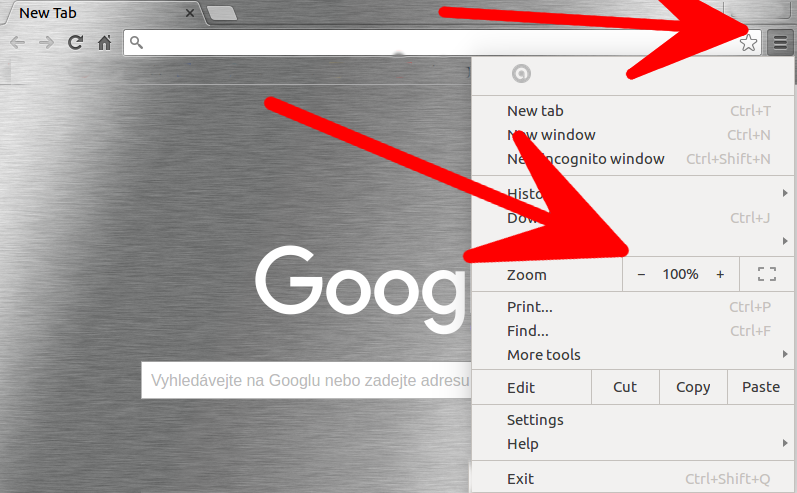
\includegraphics[width=12.5cm]{img/Chyby/zoom.png}
	\end{figure}
	
	\section{Rozměry screenshotů}
	Pokud se v~testu hledá prvek v~závislosti na pozici jiného, je možné, že nebude nalezen. Důvodem mohou být rozdílné rozměry screenshotů v~kombinaci s~použitými metodami hledání -- první prvek nalezneme, ale screenshot druhého je větší, než prohledávaná oblast vymezená rozměry prvního, tudíž nemůže být nalezen. Obrázek \ref{rozmery} demonstruje problém. Pokud budeme hledat červeně vyznačený obrázek, který je vyšší než snímek, ve kterém hledáme, nebude nalezen.
	
	\begin{figure}[ht!]
		\centering
		\caption{Nesprávné rozměry screenshotů}
		\label{rozmery}
		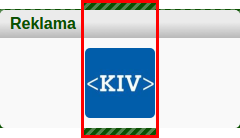
\includegraphics[width=12.5cm]{img/Chyby/reklama.png}
	\end{figure}
	
	\section{Ukazatel myši}
	Při pořizování screenshotů je vhodné vyvarovat se umístění ukazatele myši ve snímané oblasti. Ten se totiž v~průběhu testu v~této oblasti vyskytovat nemusí a~hledaný prvek by tak nemusel být rozpoznán.
	
	Stejně tak je důležité uvědomit si, že na některých platformách se simulováním pohybu myši a~klikáním mění pozice ukazatele. To může vyústit v~problém, pokud je ukazatel umístěn přes hledaný prvek, který tím pádem pravděpodobně nebude rozpoznán. Oba problémy shrnuje obrázek \ref{mys}.
	
	\begin{figure}[ht!]
		\centering
		\caption{Screenshot s ukazatelem myši}
		\label{mys}
		
\includegraphics[width=10cm]{img/Chyby/mys.png}
	\end{figure}
	
	\section{Nespolehlivé OCR}
	SikuliX poskytuje možnost rozpoznání textu v~obrázcích. Tato funkcionalita je však v~experimentální fázi a~na jejím vývoji se stále pracuje. Je tedy nespolehlivá a~pro naše účely nevhodná. Text v~obrázku buď vůbec nebyl nalezen (pokud se jednalo např. o~jedinou číslici), nebo byl špatně rozpoznán (záměna O~a~0, získána pouze část textu, apod.).
	
	Možným řešením je tedy nasimulovat korektní výstup, provést screenshot a~ten použít pro obrazové rozpoznání správného výsledku.
	
	\section{Nefunkčnost některých metod, tříd}
	Java API SikuliX poskytuje třídy a~metody pro práci s~aplikacemi a~jejich okny. Tyto metody a~třídy mají však občas jiné než očekávané chování. Vzhledem k~téměř nulové dokumentaci je toto celkem velký problém.

		\subsection{Pozice a~velikost okna}		
		Konkrétním příkladem je např. to, pokud bychom chtěli testování omezit pouze na okno aplikace. SikuliX je schopno okno s~aplikací najít podle (části) jejího titulku a~přenést jej do popředí. Už ale není schopno získat rozměry a~pozici tohoto okna, ačkoli metody pro tyto funkce existují.
	
		Postup, kterým se dá tato funkcionalita nahradit, je následující. Aplikaci najdeme podle jejího titulku a~necháme ji přenést do popředí. Poté je SikuliX schopné získat pozici a~rozměry okna, které je v~popředí (má tzv. focus), jak je ukázáno v~následujícím kódu.\\[0.2cm]
		\texttt{Region window = App.focusedWindow();\\
		Location minCoord = window.getTopLeft();\\
		Location maxCoord = window.getBottomRight();}
		
		\subsection{Stav aplikace}
		Dále nedokázalo indikovat, že aplikace skončila svůj běh. Pokud jsme tedy použili cyklus \uv{testuj, dokud aplikace běží}, testování pokračovalo i~v~případě, že byla aplikace již ukončena.
	
		Náhradním řešením tedy bylo vytvořit screenshot některé části aplikace, která se nemění a~je vždy v~aplikaci přítomna. Cyklus poté vypadá takto: \uv{testuj, dokud najdeš tuto část aplikace}. To však není řešení absolutní, protože nebude funkční v~případech, kdy se objeví např. dialogové okno, které tuto části zakryje, nebo pokud taková část vůbec neexistuje.
		
		\subsection{Spuštění aplikace}
		Metody pro spuštění aplikace \texttt{App.open("aplikace")}, \texttt{new App(\\"aplikace").open()} a~\texttt{App.run("příkaz")}, které SikuliX poskytuje, fungovaly bez problémů v~OS Linux, avšak v~OS Windows nastal problém. SikuliX nebylo schopné otevřít aplikaci pomocí žádného z~příkazů\\[0.2cm]
		\texttt{App.open("java -jar cesta/k/aplikaci.jar");\\
		new App("java -jar cesta/k/aplikaci.jar").open();\\
		App.run("java -jar cesta/k/aplikaci.jar");}\\[0.2cm]
		Týká se to pouze spouštění aplikace pomocí daného příkazu. Pokud byla zadána cesta ke spustitelnému souboru, vše proběhlo bez problémů i~za použití těchto metod.
		
		Problém jsem nebyl schopen za pomoci SikuliX vyřešit. Použil jsem proto metodu poskytovanou programovacím jazykem Java, konkrétně\\[0.2cm]
		\texttt{Runtime.getRuntime().exec("java -jar cesta/k/aplikaci.jar");\\
		App application = new App("Titulek aplikace");\\
		application.focus();}